% -------------------------------------------------------------------
% Strategy One-Pager Brief — Meridian Manufacturing Q3 FY2026 Review
% Edit and compile online at https://letx.app
% Compile: latexmk -pdf main.tex  (pdflatex, TeX Live full)
% -------------------------------------------------------------------
\documentclass[10pt,letterpaper]{article}
\usepackage{amsmath}

% === PACKAGES ===
\usepackage[table]{xcolor}
\usepackage[margin=0.45in]{geometry}
\usepackage{lato}
\renewcommand{\familydefault}{\sfdefault}
\usepackage[most]{tcolorbox}
\tcbuselibrary{skins,breakable}
\usetikzlibrary{shadows}
\usepackage{tikz}
\usepackage{pgfplots}
\pgfplotsset{compat=1.18}
\usepackage{tabularx}
\usepackage{booktabs}
\usepackage{fontawesome5}
\usepackage{enumitem}
\usepackage[explicit]{titlesec}
\usepackage{hyperref}
\hypersetup{colorlinks=true,linkcolor=navy,urlcolor=navy}

% === PAGE SETTINGS ===
\setlength{\parindent}{0pt}
\setlength{\parskip}{0pt}
\setlist{nosep,leftmargin=*}

% === COLORS ===
\definecolor{navy}{HTML}{1B2A4A}
\definecolor{gold}{HTML}{C8963E}
\definecolor{slate}{HTML}{5A6872}
\definecolor{bglight}{HTML}{F4F5F7}
\definecolor{riskred}{HTML}{C0392B}
\definecolor{accentgreen}{HTML}{1E8449}
\definecolor{softgold}{HTML}{FDF6ED}

% === TIKZ LIBRARIES ===
\usetikzlibrary{shadows,arrows.meta,positioning,calc,backgrounds}

% === HEADER BAR ===
\newtcolorbox{headerbar}{
  colback=navy, colframe=navy, boxrule=0pt,
  left=10pt, right=10pt, top=4pt, bottom=4pt,
  sharp corners, width=\textwidth,
  before skip=0pt, after skip=0pt
}

% === INSIGHT BOX ===
\newtcolorbox{insightbox}[1]{
  enhanced, colback=white, colframe=bglight,
  boxrule=0pt, left=10pt, right=10pt, top=8pt, bottom=8pt,
  sharp corners,
  overlay={
    \draw[gold, line width=2pt]
      ([yshift=2pt]frame.north west) -- ([yshift=2pt]frame.north east);
  },
  fontupper=\small, fonttitle=\bfseries\color{navy},
  title=#1
}

% === RISK CALLOUT ===
\newtcolorbox{riskcallout}{
  enhanced, colback=white, colframe=bglight,
  boxrule=0pt, left=10pt, right=10pt, top=8pt, bottom=8pt,
  sharp corners,
  borderline west={3pt}{0pt}{riskred},
  fontupper=\small
}

% === RECOMMENDATION CALLOUT ===
\newtcolorbox{reccallout}{
  enhanced, colback=softgold, colframe=gold!30,
  boxrule=0.5pt, left=10pt, right=10pt, top=8pt, bottom=8pt,
  sharp corners, arc=0pt,
  borderline west={3pt}{0pt}{gold},
  fontupper=\small
}

% === STEP BOX ===
\newtcolorbox{stepbox}[2]{
  enhanced, colback=white, colframe=navy!15,
  boxrule=0.5pt, left=8pt, right=6pt, top=6pt, bottom=6pt,
  sharp corners, arc=2pt,
  fontupper=\footnotesize,
  title={\color{navy}\bfseries\small #1},
  attach title to upper={\quad}
}

% === SECTION TITLE ===
\newcommand{\sectiontitle}[1]{%
  \vspace{2pt}%
  {\color{navy}\bfseries\footnotesize\MakeUppercase{#1}}%
  \vspace{2pt}%
}

\begin{document}

% ===================================================================
% HEADER
% ===================================================================
\begin{headerbar}
  \textcolor{white}{\footnotesize\bfseries APEX INDUSTRIAL PARTNERS}
  \hfill
  \textcolor{gold!80}{\footnotesize STRATEGY ONE-PAGER}
  \hfill
  \textcolor{white!70}{\footnotesize Q3 FY2026 \enspace$|$\enspace CONFIDENTIAL}
\end{headerbar}

\vspace{10pt}

% ===================================================================
% TITLE
% ===================================================================
{\color{navy}\LARGE\bfseries Meridian Manufacturing}
\hfill
{\color{slate}\small Portfolio Review --- October 2026}

\vspace{2pt}
{\color{gold}\rule{\textwidth}{1.5pt}}
\vspace{2pt}

\begin{minipage}[t]{0.48\textwidth}
  {\color{slate}\footnotesize Precision-engineered components for aerospace \& defense}
\end{minipage}
\begin{minipage}[t]{0.48\textwidth}
  \flushright
  \begin{tabularx}{0.55\textwidth}{@{}>{\color{navy}\bfseries\footnotesize}l@{\hspace{4mm}}>{\color{slate}\footnotesize}X@{}}
    EV              & \textdollar340M \\
    Entry           & Q1 2024 \\
    Stake           & 72\% \\
    Deal Lead       & S.\ Chen \\
  \end{tabularx}
\end{minipage}

\vspace{8pt}

% ===================================================================
% THREE KEY INSIGHTS
% ===================================================================
\begin{tcbraster}[raster columns=3, raster equal height,
                  raster column skip=6pt, raster force size=false]
\begin{insightbox}{1\enspace Margin Expansion Taking Hold}
  EBITDA margins improved \textbf{310bp} since acquisition via lean ops and
  procurement consolidation. On track for \textbf{22\% target} by Q4 FY26.
  Workforce productivity up 14\% with zero CapEx investment.
\end{insightbox}
\begin{insightbox}{2\enspace Supply Chain De-Risked}
  Dual-sourcing reduced single-supplier exposure from \textbf{64\% to 31\%}.
  Three new qualified vendors onboarded for titanium and nickel-alloy
  categories. Lead times improved by 8 days.
\end{insightbox}
\begin{insightbox}{3\enspace Aerospace Tailwinds}
  Defense backlog up \textbf{28\% YoY}; commercial MRO demand accelerating.
  Capacity utilization at \textbf{87\%} with clear path to 95\%.
  Pipeline of \$120M in qualified opportunities.
\end{insightbox}
\end{tcbraster}

\vspace{8pt}

% ===================================================================
% FINANCIAL SUMMARY + CHART
% ===================================================================
\begin{minipage}[t]{0.58\textwidth}
  \sectiontitle{Financial Summary}

  \vspace{1pt}
  \renewcommand{\arraystretch}{1.15}
  \begin{tabularx}{\linewidth}{@{}>{\color{navy}\bfseries\footnotesize}l
    @{\hspace{5mm}}
    >{\raggedright\arraybackslash\footnotesize}X
    >{\raggedleft\arraybackslash\footnotesize}p{0.18\linewidth}
    >{\raggedleft\arraybackslash\footnotesize}p{0.18\linewidth}
    >{\raggedleft\arraybackslash\footnotesize}p{0.18\linewidth}
    @{}}
    \toprule
    \rowcolor{navy!8}
    \textcolor{navy}{\textbf{Metric (\$M)}} & & \textbf{Q1 FY26} & \textbf{Q2 FY26} & \textbf{Q3 FY26} \\
    \midrule
    Revenue            & & 42.3 & 44.8 & 47.1 \\[1pt]
    Gross Profit       & & 15.7 & 16.9 & 18.0 \\[1pt]
    \textit{Gross Margin}  & & \textit{37.1\%} & \textit{37.7\%} & \textit{38.2\%} \\[1pt]
    \addlinespace
    EBITDA             & & 8.2  & 9.1  & 9.7  \\[1pt]
    \textit{EBITDA Margin} & & \textit{19.4\%} & \textit{20.3\%} & \textit{20.6\%} \\[1pt]
    \addlinespace
    Unlevered FCF      & & 3.1  & 3.8  & 4.2  \\[1pt]
    Net Debt / EBITDA  & & 3.1$\times$ & 2.9$\times$ & 2.7$\times$ \\
    \bottomrule
  \end{tabularx}

  \vspace{4pt}
  {\color{slate}\footnotesize\faIcon{arrow-up}~Revenue +\textbf{11.2\%} YoY \hspace{12pt}
   \faIcon{arrow-up}~EBITDA +\textbf{18.3\%} YoY \hspace{12pt}
   \faIcon{arrow-up}~FCF +\textbf{35.5\%} YoY}
\end{minipage}
\hfill
\begin{minipage}[t]{0.38\textwidth}
  \sectiontitle{Revenue Trend (\$M)}

  \vspace{4pt}
  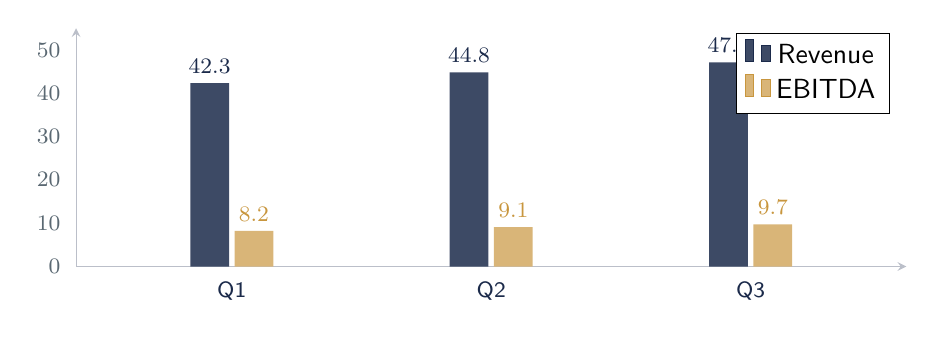
\begin{tikzpicture}
  \begin{axis}[
      width=\linewidth,
      height=0.38\textwidth,
      ybar,
      bar width=14pt,
      ymin=0, ymax=55,
      ytick={0,10,20,30,40,50},
      yticklabel style={font=\footnotesize\color{slate}},
      xtick={1,2,3},
      xticklabels={Q1, Q2, Q3},
      xticklabel style={font=\footnotesize\color{navy}},
      axis lines=left,
      axis line style={navy!30},
      tick style={draw=none},
      enlarge x limits=0.3,
      nodes near coords,
      every node near coord/.append style={
        font=\footnotesize\color{navy},
        /pgf/number format/precision=1,
        /pgf/number format/fixed
      },
    ]
    \addplot[navy, fill=navy!85, draw=none] coordinates {(1,42.3) (2,44.8) (3,47.1)};
    \addplot[gold, fill=gold!70, draw=none] coordinates {(1,8.2) (2,9.1) (3,9.7)};
    \legend{Revenue, EBITDA}
  \end{axis}
  \end{tikzpicture}

  \vspace{2pt}
  {\color{slate}\footnotesize\raggedright Target run-rate: \textbf{\$52M} quarterly revenue by Q4 FY26}
\end{minipage}

\vspace{8pt}

% ===================================================================
% RISK ASSESSMENT + RECOMMENDATION
% ===================================================================
\begin{minipage}[t]{0.48\textwidth}
  \sectiontitle{Risk Assessment}

  \vspace{2pt}
  \begin{riskcallout}
    \begin{itemize}[leftmargin=10pt, itemsep=1pt]
      \item[\color{riskred}\faExclamationTriangle]
        \textbf{Raw material exposure:} Titanium and nickel-alloy spot prices
        up 18\% since June; 40\% of COGS tied to indexed contracts.
      \item[\color{riskred}\faExclamationTriangle]
        \textbf{Customer concentration:} Top 3 accounts represent 47\% of
        revenue. Boeing renewal (32\%) expires Q1 FY27.
      \item[\color{riskred}\faExclamationTriangle]
        \textbf{Labor constraints:} Skilled CNC machinist hiring lagging plan
        by 6 FTE; overtime costs trending 2.1\% above budget.
    \end{itemize}
  \end{riskcallout}
\end{minipage}
\hfill
\begin{minipage}[t]{0.48\textwidth}
  \sectiontitle{Recommendation}

  \vspace{2pt}
  \begin{reccallout}
    \textbf{Proceed with add-on acquisition of Precision Alloys Inc.}

    \vspace{2pt}
    {\footnotesize Target EV: \textbf{\$45--55M} \enspace$|$\enspace
     Implied multiple: \textbf{6.8$\times$} LTM EBITDA}

    \vspace{3pt}
    \textbf{Rationale:}
    \begin{itemize}[leftmargin=10pt, itemsep=1pt]
      \item Vertical integration captures 200bp margin uplift
        on specialty materials.
      \item Adds 3 new Tier-1 defense customers, reducing top-3
        concentration to 38\%.
      \item Proprietary alloy IP provides 3--5 year competitive moat.
    \end{itemize}

    \vspace{2pt}
    {\footnotesize\color{accentgreen}\faCheckCircle\enspace
     Investment Committee pre-approved \$60M allocation, 19 September 2026.}
  \end{reccallout}
\end{minipage}

\vspace{10pt}

% ===================================================================
% NEXT STEPS
% ===================================================================
\sectiontitle{Next Steps}

\vspace{4pt}
\begin{tcbraster}[raster columns=4, raster equal height,
                  raster column skip=5pt, raster force size=false]
\begin{stepbox}{\makebox[14pt][l]{1}}{Immediate}
  Engage transaction counsel; issue LOI to Precision Alloys. Confirm
  committed debt financing terms with syndicate.
\end{stepbox}
\begin{stepbox}{\makebox[14pt][l]{2}}{30 Days}
  Complete confirmatory due diligence: financial, legal, IT, and
  environmental. Conduct management and site visits.
\end{stepbox}
\begin{stepbox}{\makebox[14pt][l]{3}}{60 Days}
  Finalize SPA; file HSR. Begin integration planning: ERP migration,
  procurement consolidation, org design.
\end{stepbox}
\begin{stepbox}{\makebox[14pt][l]{4}}{90 Days}
  Target close. Execute Day-1 integration playbook. Announce combined
  entity to customers and key suppliers.
\end{stepbox}
\end{tcbraster}

\vspace{6pt}

% ===================================================================
% FOOTER
% ===================================================================
{\color{gold}\rule{\textwidth}{0.6pt}}
\vspace{2pt}
{\color{slate}\footnotesize Apex Industrial Partners \textbar\ Strategy \& Operations Group
 \hfill Prepared by: S.\ Chen, M.\ Reeves \textbar\ 14 October 2026}

\end{document}
